\chapter{Results and Discussion}
The results of our experiments with our data set will be presented in this chapter. 30 runs of each approach that produced feasible solutions are included in the results. Note that some runs produce an infeasible solution. This due to the non-deterministic nature of metaheuristics, which will cause it to produce infeasible solutions sometimes.

\section{Environment}
All of the approaches were run in the following hardware and software configurations:

\begin{itemize}
	\item Hardware
	\begin{itemize}
		\item \textbf{CPU}: Intel Core i5-7400 @ 3.5GHz
		\item \textbf{GPU}: NVIDIA GeForce GTX 1050 Ti
		\item \textbf{RAM}: 8GB
	\end{itemize}
	\item Software
	\begin{itemize}
		\item \textbf{OS}: elementaryOS 5.1.7 Hera
		\item \textbf{Linux Kernel Version}: 5.4.0-74-generic
	\end{itemize}
\end{itemize}

\section{Experiments}
Each approach has their own parameters, and the values we have set for those parameters are shown in Table \ref{approach-parameters}. Both approaches use a population size of 50, and a maximum number of iterations of 400.

\begin{table}[h!]
	\centering
	\begin{tabular}{|l|l|l|}
		\hline
		\textbf{Approach}   & \textbf{Parameter} & \textbf{Value} \\ \hline
		GWO                 & c                  & 4              \\ \hline
		\multirow{3}{*}{GA} & Mutation Rate      & 0.05           \\ \cline{2-3} 
		& Tournament Size    & 4              \\ \cline{2-3} 
		& No. of Elites (EN) & 5              \\ \hline
	\end{tabular}
	\caption{Parameter values of the GWO and GA approaches.}
	\label{approach-parameters}
\end{table}

The results obtained for each approach is shown in Tables \ref{approach-ga-results} and \ref{approach-gwo-results}. As what the tables show, the competing genetic algorithm approach produces a solution that is slightly better than our proposed GWO approach, with a fitness averages of $285.678879$ and $50490.029633$ for the SFLP-II and mSFLP-III problem data sets respectively. This is compared to our proposed approach's fitness averages of $286.308150$ and $52769.171317$. For SFLP-II, the best and worst solutions were $225.564886$ and $331.295366$ for the GA, respectively, compared to our approach's $223.98231$ and $360.621471$. In this data set, our approach was capable of producing the best solution. For mSFLP-III, the best and worst solutions were $47668.453659$ and $52489.891396$ for the GA, respectively, compared to our approach's $48469.810791$ and $52489.891396$. The competing approach is also slightly more stable, basing from the the slightly lower standard deviation in both data sets, with $31.1215075$ and $1556.2861826$ for SFLP-II and mSFLP-III, respectively, compared to $36.4883564$ and $2234.4588329$ of our approach. It is also faster when SFLP-II is being used with an average run time of $30.2333333$s, compared to our approach's $69.2333333$s.

\begin{table}[h!]
\begin{adjustwidth}{-0.855in}{}
\centering
\begin{tabular}{|l|l|l|l|l|l|}
	\hline
	\multicolumn{1}{|c|}{\multirow{2}{*}{\textbf{Problem}}} & \multicolumn{5}{c|}{\textbf{Genetic Algorithm}}                                                                                                                                                                                            \\ \cline{2-6} 
	\multicolumn{1}{|c|}{}                                  & \multicolumn{1}{c|}{\textbf{Best}} & \multicolumn{1}{c|}{\textbf{Worst}} & \multicolumn{1}{c|}{\textbf{Avg.}} & \multicolumn{1}{c|}{\textbf{Std. Dev.}} & \multicolumn{1}{c|}{\textbf{Avg. Runtime (s)}} \\ \hline
	SFLP-II                                                 & 225.564886                                  & 331.295366                                   & 285.678879                      & 31.1215075                                 & 30.2333333                                   \\ \hline
	mSFLP-III                                               & 47668.453659                                & 52489.891396                                 & 50490.029633                      & 1556.2861826                                  & 260.56666667                                   \\ \hline
\end{tabular}
\end{adjustwidth}
\caption{Results obtained from using the competing GA approach.}
\label{approach-ga-results}
\end{table}

\begin{table}[h!]
\begin{adjustwidth}{-0.855in}{}
\centering
\begin{tabular}{|l|l|l|l|l|l|}
	\hline
	\multicolumn{1}{|c|}{\multirow{2}{*}{\textbf{Problem}}} & \multicolumn{5}{c|}{\textbf{Genetic Algorithm}}                                                                                                                                                                                            \\ \cline{2-6} 
	\multicolumn{1}{|c|}{}                                  & \multicolumn{1}{c|}{\textbf{Best}} & \multicolumn{1}{c|}{\textbf{Worst}} & \multicolumn{1}{c|}{\textbf{Avg.}} & \multicolumn{1}{c|}{\textbf{Std. Dev.}} & \multicolumn{1}{c|}{\textbf{Avg. Runtime (s)}} \\ \hline
	SFLP-II                                                 & 223.98231                                  & 360.621471                                   & 286.308150                      & 36.4883564                                 & 69.2333333                                   \\ \hline
	mSFLP-III                                               & 48469.810791                                & 58331.082916                                 & 52769.171317          & 2234.4588329                                  & 185.7                                   \\ \hline
\end{tabular}
\end{adjustwidth}
\caption{Results obtained from our proposed GWO approach.}
\label{approach-gwo-results}
\end{table}

Figures \ref{graph-ga-vs-gwo-sflp2} and \ref{graph-ga-vs-gwo-msflp3} show the fitness graphs of the best solutions using the SFLP-II and mSFLP-III data sets. The non-linearity of the graph of our GWO approach that is obvious in Figure \ref{graph-ga-vs-gwo-sflp2} is due to the nature of our approach. All solutions in a population are replaced. Hence, the best solutions may be replaced by poorer solutions. This characteristic is not as obvious in Figure \ref{graph-ga-vs-gwo-msflp3}. In Figure \ref{graph-ga-vs-gwo-sflp2} with the SFLP-II data set, the GA approach converges was than the GWO approach. This is due to how our approach replaces all solutions in the population for the next iteration. The size of the bounding region in SFLP-II may also be reason as it does not have a huge space for our approach to move buildings in various directions and prevent intersections as much as possible. This is the different from the mSFLP-III where the bounding region is larger, allowing buildings to less likely intersect with one another. Figure \ref{graph-ga-vs-gwo-msflp3} showcases the behaviour of our GWO approach with a larger bounding region.

\begin{figure}[h!]
\centering
\begin{adjustwidth}{-0.9in}{}
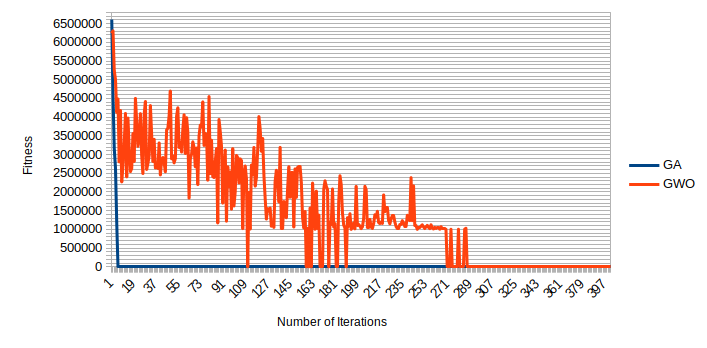
\includegraphics[scale=0.75]{./images/chap07-rd/gwo-sflp2-graph.png}
\end{adjustwidth}
\caption{Fitness graph of the best solutions of the competing GA approach, and our GWO approach using the SFLP-II data set.}
\label{graph-ga-vs-gwo-sflp2}
\end{figure}

\begin{figure}[h!]
\centering
\begin{adjustwidth}{-0.1in}{}
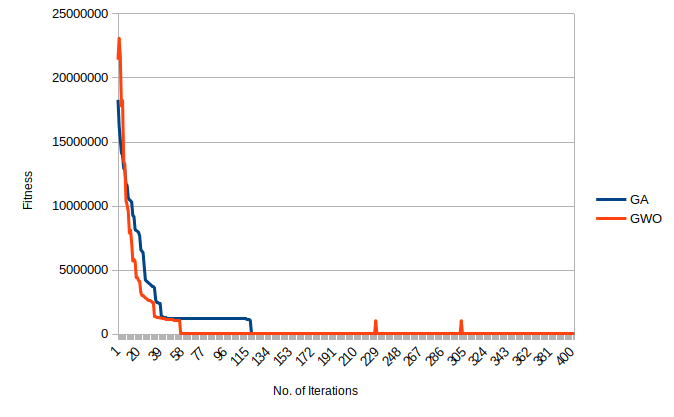
\includegraphics[scale=0.65]{./images/chap07-rd/gwo-msflp3-graph.png}
\end{adjustwidth}
\caption{Fitness graph of the best solutions of the competing GA approach, and our GWO approach using the mSFLP-III data set.}
\label{graph-ga-vs-gwo-msflp3}
\end{figure}

% TODO: Add figure of best generated solutions.

Despite the wins showcased by the competing GA approach, our proposed approach is faster when mSFLP-III is used with $185.7$s for our approach, while the GA approach takes $260.56666667$s. We also argue that the competing approach is already a hybridized approach with phases for a local search to be performed. Our approach can be considered to be a relatively pure adaptation of classical GWO, rather than a hybrid approach. Additionally, the results are not far from the results generated by the competing approach. They show that the simplicity of our approach (which only uses three parameters needed, compared to our competing approach's six) does not prevent our proposed algorithm from almost reaching competitiveness. They also indicate that there is promise in further exploring the applicability of the grey wolf optimization algorithm in the facility layout problem.

